
%% bare_jrnl_compsoc.tex
%% V1.4b
%% 2015/08/26
%% by Michael Shell
%% See:
%% http://www.michaelshell.org/
%% for current contact information.
%%
%% This is a skeleton file demonstrating the use of IEEEtran.cls
%% (requires IEEEtran.cls version 1.8b or later) with an IEEE
%% Computer Society journal paper
%%
%% Support sites:
%% http://www.michaelshell.org/tex/ieeetran/
%% http://www.ctan.org/pkg/ieeetran
%% and
%% http://www.ieee.org/

%%*************************************************************************
%% Legal Notice:
%% This code is offered as-is without any warranty either expressed or
%% implied; without even the implied warranty of MERCHANTABILITY or
%% FITNESS FOR A PARTICULAR PURPOSE! 
%% User assumes all risk.
%% In no event shall the IEEE or any contributor to this code be liable for
%% any damages or losses, including, but not limited to, incidental,
%% consequential, or any other damages, resulting from the use or misuse
%% of any information contained here.
%%
%% All comments are the opinions of their respective authors and are not
%% necessarily endorsed by the IEEE.
%%
%% This work is distributed under the LaTeX Project Public License (LPPL)
%% ( http://www.latex-project.org/ ) version 1.3, and may be freely used,
%% distributed and modified. A copy of the LPPL, version 1.3, is included
%% in the base LaTeX documentation of all distributions of LaTeX released
%% 2003/12/01 or later.
%% Retain all contribution notices and credits.
%% ** Modified files should be clearly indicated as such, including  **
%% ** renaming them and changing author support contact information. **
%%*************************************************************************


% *** Authors should verify (and, if needed, correct) their LaTeX system  ***
% *** with the testflow diagnostic prior to trusting their LaTeX platform ***
% *** with production work. The IEEE's font choices and paper sizes can   ***
% *** trigger bugs that do not appear when using other class files.       ***                          ***
% The testflow support page is at:
% http://www.michaelshell.org/tex/testflow/


\documentclass[10pt,journal,compsoc]{IEEEtran}
%
% If IEEEtran.cls has not been installed into the LaTeX system files,
% manually specify the path to it like:
% \documentclass[10pt,journal,compsoc]{../sty/IEEEtran}





% Some very useful LaTeX packages include:
% (uncomment the ones you want to load)


% *** MISC UTILITY PACKAGES ***
%
%\usepackage{ifpdf}
% Heiko Oberdiek's ifpdf.sty is very useful if you need conditional
% compilation based on whether the output is pdf or dvi.
% usage:
% \ifpdf
%   % pdf code
% \else
%   % dvi code
% \fi
% The latest version of ifpdf.sty can be obtained from:
% http://www.ctan.org/pkg/ifpdf
% Also, note that IEEEtran.cls V1.7 and later provides a builtin
% \ifCLASSINFOpdf conditional that works the same way.
% When switching from latex to pdflatex and vice-versa, the compiler may
% have to be run twice to clear warning/error messages.






% *** CITATION PACKAGES ***
%
\ifCLASSOPTIONcompsoc
  % IEEE Computer Society needs nocompress option
  % requires cite.sty v4.0 or later (November 2003)
  \usepackage[nocompress]{cite}
\else
  % normal IEEE
  \usepackage{cite}
\fi
% cite.sty was written by Donald Arseneau
% V1.6 and later of IEEEtran pre-defines the format of the cite.sty package
% \cite{} output to follow that of the IEEE. Loading the cite package will
% result in citation numbers being automatically sorted and properly
% "compressed/ranged". e.g., [1], [9], [2], [7], [5], [6] without using
% cite.sty will become [1], [2], [5]--[7], [9] using cite.sty. cite.sty's
% \cite will automatically add leading space, if needed. Use cite.sty's
% noadjust option (cite.sty V3.8 and later) if you want to turn this off
% such as if a citation ever needs to be enclosed in parenthesis.
% cite.sty is already installed on most LaTeX systems. Be sure and use
% version 5.0 (2009-03-20) and later if using hyperref.sty.
% The latest version can be obtained at:
% http://www.ctan.org/pkg/cite
% The documentation is contained in the cite.sty file itself.
%
% Note that some packages require special options to format as the Computer
% Society requires. In particular, Computer Society  papers do not use
% compressed citation ranges as is done in typical IEEE papers
% (e.g., [1]-[4]). Instead, they list every citation separately in order
% (e.g., [1], [2], [3], [4]). To get the latter we need to load the cite
% package with the nocompress option which is supported by cite.sty v4.0
% and later. Note also the use of a CLASSOPTION conditional provided by
% IEEEtran.cls V1.7 and later.



\usepackage{xcolor}
\newcommand{\m}{\textcolor{red}}


% *** GRAPHICS RELATED PACKAGES ***
%
\ifCLASSINFOpdf
  % \usepackage[pdftex]{graphicx}
  % declare the path(s) where your graphic files are
  % \graphicspath{{../pdf/}{../jpeg/}}
  % and their extensions so you won't have to specify these with
  % every instance of \includegraphics
  % \DeclareGraphicsExtensions{.pdf,.jpeg,.png}
\else
  % or other class option (dvipsone, dvipdf, if not using dvips). graphicx
  % will default to the driver specified in the system graphics.cfg if no
  % driver is specified.
  % \usepackage[dvips]{graphicx}
  % declare the path(s) where your graphic files are
  % \graphicspath{{../eps/}}
  % and their extensions so you won't have to specify these with
  % every instance of \includegraphics
  % \DeclareGraphicsExtensions{.eps}
\fi
% graphicx was written by David Carlisle and Sebastian Rahtz. It is
% required if you want graphics, photos, etc. graphicx.sty is already
% installed on most LaTeX systems. The latest version and documentation
% can be obtained at: 
% http://www.ctan.org/pkg/graphicx
% Another good source of documentation is "Using Imported Graphics in
% LaTeX2e" by Keith Reckdahl which can be found at:
% http://www.ctan.org/pkg/epslatex
%
% latex, and pdflatex in dvi mode, support graphics in encapsulated
% postscript (.eps) format. pdflatex in pdf mode supports graphics
% in .pdf, .jpeg, .png and .mps (metapost) formats. Users should ensure
% that all non-photo figures use a vector format (.eps, .pdf, .mps) and
% not a bitmapped formats (.jpeg, .png). The IEEE frowns on bitmapped formats
% which can result in "jaggedy"/blurry rendering of lines and letters as
% well as large increases in file sizes.
%
% You can find documentation about the pdfTeX application at:
% http://www.tug.org/applications/pdftex


\usepackage{graphicx}
\usepackage{algorithm}% http://ctan.org/pkg/algorithm
\usepackage{algpseudocode}% http://ctan.

\usepackage{multirow}
\usepackage{tabularx}

% *** MATH PACKAGES ***
%
%\usepackage{amsmath}
% A popular package from the American Mathematical Society that provides
% many useful and powerful commands for dealing with mathematics.
%
% Note that the amsmath package sets \interdisplaylinepenalty to 10000
% thus preventing page breaks from occurring within multiline equations. Use:
%\interdisplaylinepenalty=2500
% after loading amsmath to restore such page breaks as IEEEtran.cls normally
% does. amsmath.sty is already installed on most LaTeX systems. The latest
% version and documentation can be obtained at:
% http://www.ctan.org/pkg/amsmath





% *** SPECIALIZED LIST PACKAGES ***
%
%\usepackage{algorithmic}
% algorithmic.sty was written by Peter Williams and Rogerio Brito.
% This package provides an algorithmic environment fo describing algorithms.
% You can use the algorithmic environment in-text or within a figure
% environment to provide for a floating algorithm. Do NOT use the algorithm
% floating environment provided by algorithm.sty (by the same authors) or
% algorithm2e.sty (by Christophe Fiorio) as the IEEE does not use dedicated
% algorithm float types and packages that provide these will not provide
% correct IEEE style captions. The latest version and documentation of
% algorithmic.sty can be obtained at:
% http://www.ctan.org/pkg/algorithms
% Also of interest may be the (relatively newer and more customizable)
% algorithmicx.sty package by Szasz Janos:
% http://www.ctan.org/pkg/algorithmicx




% *** ALIGNMENT PACKAGES ***
%
%\usepackage{array}
% Frank Mittelbach's and David Carlisle's array.sty patches and improves
% the standard LaTeX2e array and tabular environments to provide better
% appearance and additional user controls. As the default LaTeX2e table
% generation code is lacking to the point of almost being broken with
% respect to the quality of the end results, all users are strongly
% advised to use an enhanced (at the very least that provided by array.sty)
% set of table tools. array.sty is already installed on most systems. The
% latest version and documentation can be obtained at:
% http://www.ctan.org/pkg/array


% IEEEtran contains the IEEEeqnarray family of commands that can be used to
% generate multiline equations as well as matrices, tables, etc., of high
% quality.




% *** SUBFIGURE PACKAGES ***
%\ifCLASSOPTIONcompsoc
%  \usepackage[caption=false,font=footnotesize,labelfont=sf,textfont=sf]{subfig}
%\else
%  \usepackage[caption=false,font=footnotesize]{subfig}
%\fi
% subfig.sty, written by Steven Douglas Cochran, is the modern replacement
% for subfigure.sty, the latter of which is no longer maintained and is
% incompatible with some LaTeX packages including fixltx2e. However,
% subfig.sty requires and automatically loads Axel Sommerfeldt's caption.sty
% which will override IEEEtran.cls' handling of captions and this will result
% in non-IEEE style figure/table captions. To prevent this problem, be sure
% and invoke subfig.sty's "caption=false" package option (available since
% subfig.sty version 1.3, 2005/06/28) as this is will preserve IEEEtran.cls
% handling of captions.
% Note that the Computer Society format requires a sans serif font rather
% than the serif font used in traditional IEEE formatting and thus the need
% to invoke different subfig.sty package options depending on whether
% compsoc mode has been enabled.
%
% The latest version and documentation of subfig.sty can be obtained at:
% http://www.ctan.org/pkg/subfig




% *** FLOAT PACKAGES ***
%
%\usepackage{fixltx2e}
% fixltx2e, the successor to the earlier fix2col.sty, was written by
% Frank Mittelbach and David Carlisle. This package corrects a few problems
% in the LaTeX2e kernel, the most notable of which is that in current
% LaTeX2e releases, the ordering of single and double column floats is not
% guaranteed to be preserved. Thus, an unpatched LaTeX2e can allow a
% single column figure to be placed prior to an earlier double column
% figure.
% Be aware that LaTeX2e kernels dated 2015 and later have fixltx2e.sty's
% corrections already built into the system in which case a warning will
% be issued if an attempt is made to load fixltx2e.sty as it is no longer
% needed.
% The latest version and documentation can be found at:
% http://www.ctan.org/pkg/fixltx2e


%\usepackage{stfloats}
% stfloats.sty was written by Sigitas Tolusis. This package gives LaTeX2e
% the ability to do double column floats at the bottom of the page as well
% as the top. (e.g., "\begin{figure*}[!b]" is not normally possible in
% LaTeX2e). It also provides a command:
%\fnbelowfloat
% to enable the placement of footnotes below bottom floats (the standard
% LaTeX2e kernel puts them above bottom floats). This is an invasive package
% which rewrites many portions of the LaTeX2e float routines. It may not work
% with other packages that modify the LaTeX2e float routines. The latest
% version and documentation can be obtained at:
% http://www.ctan.org/pkg/stfloats
% Do not use the stfloats baselinefloat ability as the IEEE does not allow
% \baselineskip to stretch. Authors submitting work to the IEEE should note
% that the IEEE rarely uses double column equations and that authors should try
% to avoid such use. Do not be tempted to use the cuted.sty or midfloat.sty
% packages (also by Sigitas Tolusis) as the IEEE does not format its papers in
% such ways.
% Do not attempt to use stfloats with fixltx2e as they are incompatible.
% Instead, use Morten Hogholm'a dblfloatfix which combines the features
% of both fixltx2e and stfloats:
%
% \usepackage{dblfloatfix}
% The latest version can be found at:
% http://www.ctan.org/pkg/dblfloatfix




%\ifCLASSOPTIONcaptionsoff
%  \usepackage[nomarkers]{endfloat}
% \let\MYoriglatexcaption\caption
% \renewcommand{\caption}[2][\relax]{\MYoriglatexcaption[#2]{#2}}
%\fi
% endfloat.sty was written by James Darrell McCauley, Jeff Goldberg and 
% Axel Sommerfeldt. This package may be useful when used in conjunction with 
% IEEEtran.cls'  captionsoff option. Some IEEE journals/societies require that
% submissions have lists of figures/tables at the end of the paper and that
% figures/tables without any captions are placed on a page by themselves at
% the end of the document. If needed, the draftcls IEEEtran class option or
% \CLASSINPUTbaselinestretch interface can be used to increase the line
% spacing as well. Be sure and use the nomarkers option of endfloat to
% prevent endfloat from "marking" where the figures would have been placed
% in the text. The two hack lines of code above are a slight modification of
% that suggested by in the endfloat docs (section 8.4.1) to ensure that
% the full captions always appear in the list of figures/tables - even if
% the user used the short optional argument of \caption[]{}.
% IEEE papers do not typically make use of \caption[]'s optional argument,
% so this should not be an issue. A similar trick can be used to disable
% captions of packages such as subfig.sty that lack options to turn off
% the subcaptions:
% For subfig.sty:
% \let\MYorigsubfloat\subfloat
% \renewcommand{\subfloat}[2][\relax]{\MYorigsubfloat[]{#2}}
% However, the above trick will not work if both optional arguments of
% the \subfloat command are used. Furthermore, there needs to be a
% description of each subfigure *somewhere* and endfloat does not add
% subfigure captions to its list of figures. Thus, the best approach is to
% avoid the use of subfigure captions (many IEEE journals avoid them anyway)
% and instead reference/explain all the subfigures within the main caption.
% The latest version of endfloat.sty and its documentation can obtained at:
% http://www.ctan.org/pkg/endfloat
%
% The IEEEtran \ifCLASSOPTIONcaptionsoff conditional can also be used
% later in the document, say, to conditionally put the References on a 
% page by themselves.




% *** PDF, URL AND HYPERLINK PACKAGES ***
%
%\usepackage{url}
% url.sty was written by Donald Arseneau. It provides better support for
% handling and breaking URLs. url.sty is already installed on most LaTeX
% systems. The latest version and documentation can be obtained at:
% http://www.ctan.org/pkg/url
% Basically, \url{my_url_here}.





% *** Do not adjust lengths that control margins, column widths, etc. ***
% *** Do not use packages that alter fonts (such as pslatex).         ***
% There should be no need to do such things with IEEEtran.cls V1.6 and later.
% (Unless specifically asked to do so by the journal or conference you plan
% to submit to, of course. )


% correct bad hyphenation here
\hyphenation{op-tical net-works semi-conduc-tor}


\begin{document}
%
% paper title
% Titles are generally capitalized except for words such as a, an, and, as,
% at, but, by, for, in, nor, of, on, or, the, to and up, which are usually
% not capitalized unless they are the first or last word of the title.
% Linebreaks \\ can be used within to get better formatting as desired.
% Do not put math or special symbols in the title.
\title{ Whose City? City Folding: Visual Exploration of Urban Dynamics based on Diverse Deomgraphics}

%Visual Object Interaction, Interaction on Visual Objects, 

%
%
% author names and IEEE memberships
% note positions of commas and nonbreaking spaces ( ~ ) LaTeX will not break
% a structure at a ~ so this keeps an author's name from being broken across
% two lines.
% use \thanks{} to gain access to the first footnote area
% a separate \thanks must be used for each paragraph as LaTeX2e's \thanks
% was not built to handle multiple paragraphs
%
%
%\IEEEcompsocitemizethanks is a special \thanks that produces the bulleted
% lists the Computer Society journals use for "first footnote" author
% affiliations. Use \IEEEcompsocthanksitem which works much like \item
% for each affiliation group. When not in compsoc mode,
% \IEEEcompsocitemizethanks becomes like \thanks and
% \IEEEcompsocthanksitem becomes a line break with idention. This
% facilitates dual compilation, although admittedly the differences in the
% desired content of \author between the different types of papers makes a
% one-size-fits-all approach a daunting prospect. For instance, compsoc 
% journal papers have the author affiliations above the "Manuscript
% received ..."  text while in non-compsoc journals this is reversed. Sigh.

% \author{Min Lu 
% Jie Liang% <-this % stops a space
% \IEEEcompsocitemizethanks{\IEEEcompsocthanksitem Min Lu is with the ShenZhen University. E-mail: minlu@szu.edu.cn
% % note need leading \protect in front of \\ to get a newline within \thanks as
% % \\ is fragile and will error, could use \hfil\break instead.
% \IEEEcompsocthanksitem Jie Liang is with The University of Technology, Sydney, Australia. E-mail: jie.liang@uts.edu.au
% \IEEEcompsocthanksitem Yu Zhang is with the Oxford University. E-mail: yuzhang94@pku.edu.cn% <-this % stops an unwanted space
% \IEEEcompsocthanksitem Yu Zhang is with the Oxford University. E-mail: yuzhang94@pku.edu.cn
% \thanks{Manuscript received April 19, 2005; revised August 26, 2015.}}

\author{ %
\IEEEcompsocitemizethanks{
\IEEEcompsocthanksitem ... 
}
%\protect\\

% note need leading \protect in front of \\ to get a newline within \thanks as
% \\ is fragile and will error, could use \hfil\break instead.
%\IEEEcompsocthanksitem J. Doe and J. Doe are with Anonymous University.}% <-this % stops an unwanted space
\thanks{Manuscript received November 30, 2017}}

% note the % following the last \IEEEmembership and also \thanks - 
% these prevent an unwanted space from occurring between the last author name
% and the end of the author line. i.e., if you had this:
% 
% \author{....lastname \thanks{...} \thanks{...} }
%                     ^------------^------------^----Do not want these spaces!
%
% a space would be appended to the last name and could cause every name on that
% line to be shifted left slightly. This is one of those "LaTeX things". For
% instance, "\textbf{A} \textbf{B}" will typeset as "A B" not "AB". To get
% "AB" then you have to do: "\textbf{A}\textbf{B}"
% \thanks is no different in this regard, so shield the last } of each \thanks
% that ends a line with a % and do not let a space in before the next \thanks.
% Spaces after \IEEEmembership other than the last one are OK (and needed) as
% you are supposed to have spaces between the names. For what it is worth,
% this is a minor point as most people would not even notice if the said evil
% space somehow managed to creep in.



% The paper headers
\markboth{Journal of \LaTeX\ Class Files,~Vol.~14, No.~8, August~2015}%
{Shell \MakeLowercase{\textit{et al.}}: Bare Demo of IEEEtran.cls for Computer Society Journals}
% The only time the second header will appear is for the odd numbered pages
% after the title page when using the twoside option.
% 
% *** Note that you probably will NOT want to include the author's ***
% *** name in the headers of peer review papers.                   ***
% You can use \ifCLASSOPTIONpeerreview for conditional compilation here if
% you desire.



% The publisher's ID mark at the bottom of the page is less important with
% Computer Society journal papers as those publications place the marks
% outside of the main text columns and, therefore, unlike regular IEEE
% journals, the available text space is not reduced by their presence.
% If you want to put a publisher's ID mark on the page you can do it like
% this:
%\IEEEpubid{0000--0000/00\$00.00~\copyright~2015 IEEE}
% or like this to get the Computer Society new two part style.
%\IEEEpubid{\makebox[\columnwidth]{\hfill 0000--0000/00/\$00.00~\copyright~2015 IEEE}%
%\hspace{\columnsep}\makebox[\columnwidth]{Published by the IEEE Computer Society\hfill}}
% Remember, if you use this you must call \IEEEpubidadjcol in the second
% column for its text to clear the IEEEpubid mark (Computer Society jorunal
% papers don't need this extra clearance.)



% use for special paper notices
%\IEEEspecialpapernotice{(Invited Paper)}



% for Computer Society papers, we must declare the abstract and index terms
% PRIOR to the title within the \IEEEtitleabstractindextext IEEEtran
% command as these need to go into the title area created by \maketitle.
% As a general rule, do not put math, special symbols or citations
% in the abstract or keywords.
\IEEEtitleabstractindextext{%
\begin{abstract}

A city is shaped not only by its natural geographic landscape but also its people with different social characteristics. Compared to the analysis of anomonous urban activities, analysis of urban dynamics in the context of individual profiles is limited to the conventional demographicl field, which is performed less frequently to the e-speed nowdays. In this work, we propose a visual analytics system of urban dynamics of people with modelled individual characteristics, to explore the accessiblity and activity and visualize the pheonomenon of city folding to different people in different levels of social attributes (e.g., income, education, etc). A data-driven profile visualization provides intuitive visual clues to help users with the identification of individuals. Back up by an classification and geo-temporal clustering algorithms, a visualization in 2.5D space shows the up and down regions of a single class. ...

Character a city with flows of people with individual characteristics.

imply the social-spatial distributions within cities

\end{abstract}

% Note that keywords are not normally used for peerreview papers.
\begin{IEEEkeywords}
Demographics, Spatial-temporal Visualization,
\end{IEEEkeywords}}


% make the title area
\maketitle


% To allow for easy dual compilation without having to reenter the
% abstract/keywords data, the \IEEEtitleabstractindextext text will
% not be used in maketitle, but will appear (i.e., to be "transported")
% here as \IEEEdisplaynontitleabstractindextext when the compsoc 
% or transmag modes are not selected <OR> if conference mode is selected 
% - because all conference papers position the abstract like regular
% papers do.
\IEEEdisplaynontitleabstractindextext
% \IEEEdisplaynontitleabstractindextext has no effect when using
% compsoc or transmag under a non-conference mode.



% For peer review papers, you can put extra information on the cover
% page as needed:
% \ifCLASSOPTIONpeerreview
% \begin{center} \bfseries EDICS Category: 3-BBND \end{center}
% \fi
%
% For peerreview papers, this IEEEtran command inserts a page break and
% creates the second title. It will be ignored for other modes.
\IEEEpeerreviewmaketitle



\IEEEraisesectionheading{\section{Introduction}\label{sec:introduction}}
% Computer Society journal (but not conference!) papers do something unusual
% with the very first section heading (almost always called "Introduction").
% They place it ABOVE the main text! IEEEtran.cls does not automatically do
% this for you, but you can achieve this effect with the provided
% \IEEEraisesectionheading{} command. Note the need to keep any \label that
% is to refer to the section immediately after \section in the above as
% \IEEEraisesectionheading puts \section within a raised box.




% The very first letter is a 2 line initial drop letter followed
% by the rest of the first word in caps (small caps for compsoc).
% 
% form to use if the first word consists of a single letter:
% \IEEEPARstart{A}{demo} file is ....
% 
% form to use if you need the single drop letter followed by
% normal text (unknown if ever used by the IEEE):
% \IEEEPARstart{A}{}demo file is ....
% 
% Some journals put the first two words in caps:
% \IEEEPARstart{T}{his demo} file is ....
% 
% Here we have the typical use of a "T" for an initial drop letter
% and "HIS" in caps to complete the first word.

% \IEEEPARstart{O}{verdrawing} scatterplot is ...
City is shaped by accessibility. Activity of people is constrained by social attributes. City planning is to relax the space which would activate the city... (Look for some statement in paper about the importance of community diversity). Back to 1970, Pahl~\cite{pahl1975whose} raised the question `whose city` and interest in understanding the territorial ineuqalities and social exclusions in his thesis. Contemporal contestation also continuely raries the question of `whose city`, demonad in the access to the city
 ~\cite{Mayer2017_whosecity}, urge to have a understanding of how ... 


In many work, anonymous movement data reveal the overall travel behaviour without social characteristics... More literature introduces...Urban infrastructure centered, roads, regions are studied. Peopole centered, most related work is social media based, By considering people as the mobile sensor, about certain topics/keywords it is also an indirect way. 

Because social characteristics is private that not easy to get. (Emphasize how special our research is). We conduct an online demographical colleciton campaign based on famouse social medial platform. With the wide-use of mobile device. Collecting data via a widely used social medial platform, users (what the right word here?) with various profiles are reached and assembled as rich (and fair?) demographic data. (what we are going to do)

In this work, we contextualize the analysis of urban dynamics in the backcloth of demographcis experiment. With a performed demographics survey via social media, our motivation is to mine this source in an attempt to ascentain the dynamics pattern of flows with different social characteristics. For this, we propose a visual analytics system People Centered. Interactive Classification Method, Movement Clustering Algorithm, A visual method about data driven semnatic visual profile drawing, 2.5 Spatial Exploration. ...
We believe this work to be one of the nature steps into research of social understanding of the city. 


% You must have at least 2 lines in the paragraph with the drop letter
% (should never be an issue)

\section{Related Work}

This work concerns to the research topic of spatial data visual analytics. Spatio-temporal data has three components, i.e., spatial, temporal and thematic~\cite{andrienko2013visual}. Lots of related work focus on the spatio-temporal analysis in movement data, in the absence of thematic information. The presense of geo-tagged social media data flourishes the exploration of thematic information along with movement. By analyzing the texts, those work explain what drive the moving activities or what is resulted from. This work continues the thematic research in movement data, but focus more on individual charecteristics. Landed by a census experiment, this work is able to analyze the profile information directly, to get rid of indirect data inferred from social media data as other related work do.

\textbf{Movement Data Analysis} 
 
 With the development of location-acquistion techniques, massive spatial trajectories are collected, to keep track of the trajectories of various moving objects. Many techniques have been proposed to process, mining trajectory~\cite{Zheng2015_trajectory}. In the field of visualization and visual analytic, spatial visualizations are specifically designed for the time, locations, spatial-temporal information and other properties in the traffic data~\cite{chen2015survey}. A large number of visual analytics tools and applications cover situation-aware exploration, pattern discovery and traffic situation monitoring. Wang et al~\cite{wang2013visual} extract the traffic jam propagation graph extraction to reveal underlying data patterns. Guo et al.~\cite{guo2011tripvista} and Zeng et al.~\cite{zeng2013visualizing} et al. construct geographical regions and visually aggregate the in-between movements as flows. To discover the route travel patterns, Lu et al.~\cite{lu2015trajrank} propose TrajRank to explore the route travel behaviour based on ranking. For multiple routes, Liu et al.~\cite{liu2011_routediversity} study the route diversity between locations and Lu et al.~\cite{Lu2017_multipleroute} explore the route choice behaviour among multiple routes.


\textbf{Geo-tagged Social Media Data Analysis}

As the prevence of social medial serivces, social media data with geo-tags are collected to track people's movements in daily lifes. As an analogue of remote sensing data in social science research, the geospatial big data has been proposed as social sensing ~\cite{liu2015social}. Hence, analyzing movement information along with rich text has become a hot research area in recent years. Those works infer thematic information from the semantic texts. Cao et al.~\cite{cao2012whisper} propose \textit{Whisper} for tracing the pathways of tweets on a spatial hierarchical layouts, to investigate how information flow among multiple places. Krueger et al.~\cite{krueger2014visual} used GPS and location-based service data to support the analysis of movement behaviors. Chen et al.~\cite{chen2016interactive} present a visual analytics system to support the exploraiton of sparcely sampled trajectory from social media. Some other researches tend to infer real information, such as names, gender, etc~\cite{peddinti2014internet}, to break down the demographic characteristics of social media users. Luo et al.~\cite{luo2016explore} derive race, gender and age as three demographics dimensions to analyze its impact on the urban human mobility patterns. Since real information is not enforced in social media, wrong infering is inevitable. Longley et al.~\cite{Longley2015}~\cite{Paul2016_twitter} identifies and assess the biases inherent in social media usage in social research and evaluate the deployment of social media data in research applications.  








\section{Data}

The advent of mobile sensing techniques makes it possible to develop urban geography from social media source. Complement the conventional census, social media brings the benefit of larger sampling frequency and higher disaggregate in terms of space and time, which reaches a wide range of individuals as well as collects the movement in human inactive time, such as the mid-night.

By Wechat, a widely used social media app we deployed the data collecting experiment in Shenzhen, one of the modernest metropolis in China. Figure~\ref{fig:app} shows the interfaces of the collecting app. Each individual hands in his or her personal characteristics from social, economic and deomgraphic aspects. For privacy issue, all detailed personal information are desensitized to categorical levels (Figure~\ref{fig:app}(b)). Also, individual is encouraged to upload trips (Figure~\ref{fig:app}(c)), including the information of start/end location and time, the traveling purpose and modes. A credit system is built up to retain the trip contribution of individuals and rewards those in the top contribution list (Figure~\ref{fig:app}(d)). 

\begin{figure}[htb!]
 \centering % avoid the use of \begin{center}...\end{center} and use \centering instead (more compact)
 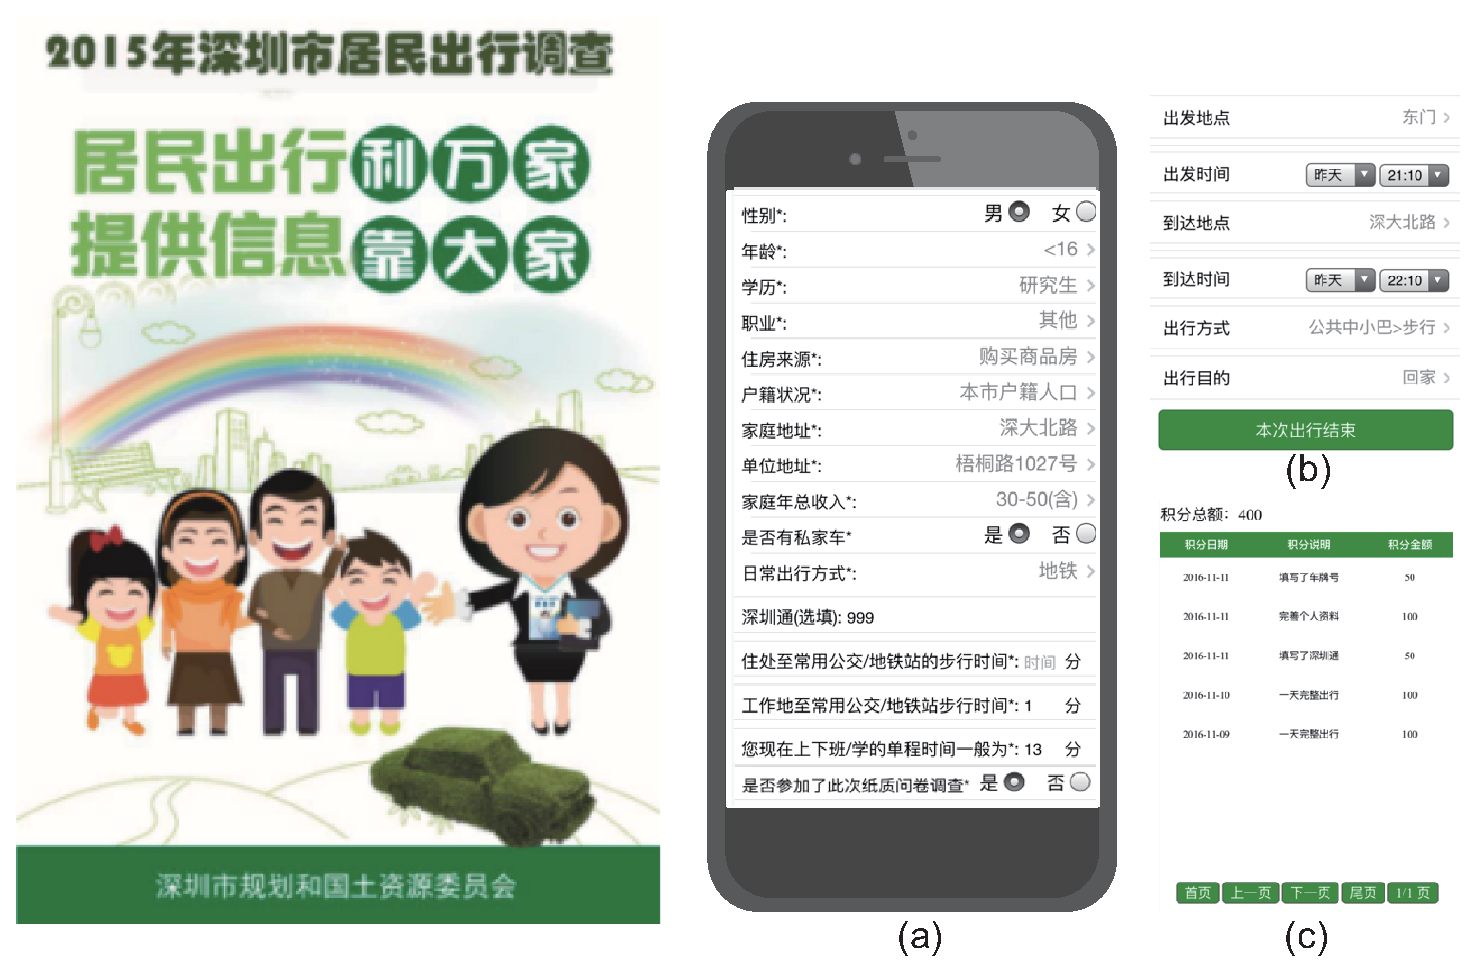
\includegraphics[width=\columnwidth]{pictures/survey_app}
 \caption{Collecting Interface: (a) welcome page; (b) personal characteristics collecting page; (c) trips collecting page; (d) credit system page}
 \label{fig:app}
\end{figure}


Over the releasing time period from June to October in 2015, 25481 individules were reached and XXX trips are collected, XX trips per individual. Figure~\ref{fig:data_over} lists the XX variables, falling into 8 domains. Those domains give a generalized depiction of the individual characteristics and serve as the ingredients for the analysis of urban dynamics over diverse people. 

Considering the caveat that self-selecting individuals are most unlikely to represent any clearly defined population~\cite{Longley2015}, a series of statistical analysis is performed to check whether it is rich enough to represent a wide range of human individuals in the city.


\begin{figure}[htb!]
 \centering % avoid the use of \begin{center}...\end{center} and use \centering instead (more compact)
 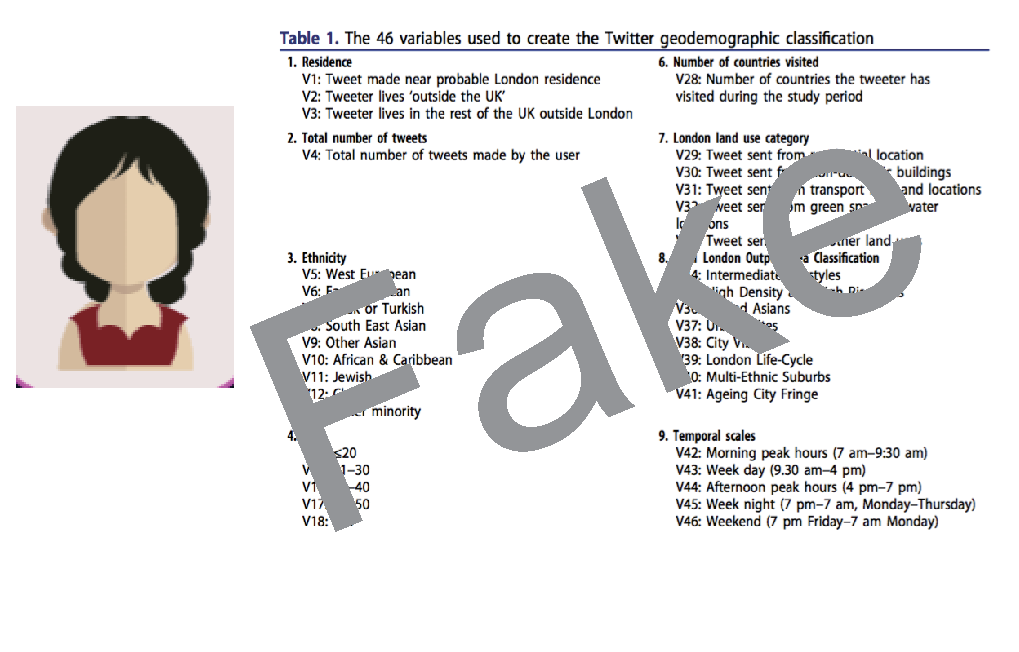
\includegraphics[width=\columnwidth]{pictures/data_over}
 \caption{Profile of Individual: XX variables falling into 8 domains enriches the analysis of urban dynamics}
 \label{fig:data_over}
\end{figure}

According to the 2015 Annual Census Statistics report~\footnote{http://www.sztj.gov.cn/xxgk/tjsj/pcgb/201606/t20160614\_3697000.htm}, people aging 15-64 occupy 83.23\% and the median age is 31.5. Shenzhen is majority of young people. 

\textit{Overview} Figure~\ref{fig:data_stat} shows samples covering almost all ages and age between 18 to 45. The 

\textit{Compared to Census} In the report (looking for some report), the penetration of mobile device is XXX, almost every XX people got a Mobile Phone in the urban. XX.  multiple social characteristics of a people is sampled, including income, education, etc. age and income distribution follows the social architecture. 


\begin{figure}[htb!]
 \centering % avoid the use of \begin{center}...\end{center} and use \centering instead (more compact)
 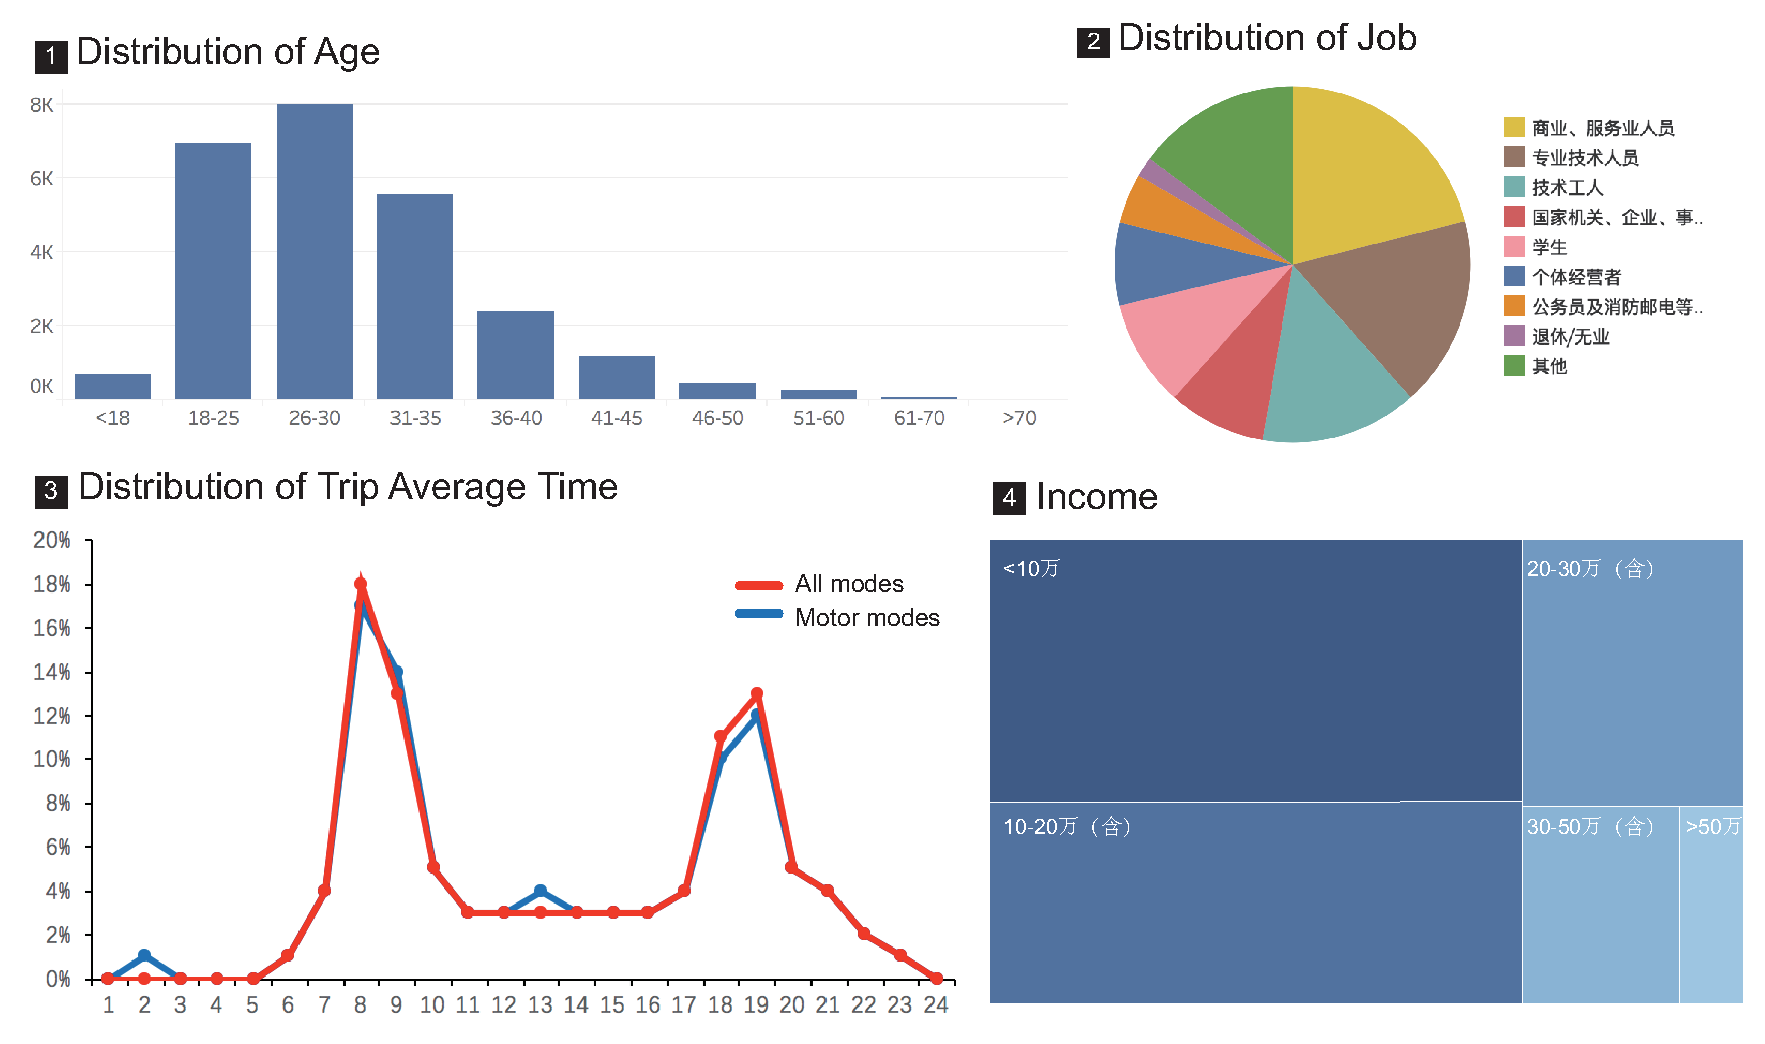
\includegraphics[width=\columnwidth]{pictures/data_detail}
 \caption{Statistical Overview of Social Characteristics}
 \label{fig:data_stat}
\end{figure}



\section{System Design}


This work we try to answer following questions:

Problem to solve: 
\begin{itemize}
\item \textit{What flows of people with certain demographic characteristics}: multiple attributes, semantic understanding, loose attribute boundary
\item \textit{What the Urban Dynamics of the Group}: where those people go and how they access the ... in a city. the patterns of behaviour classified by different social characteristics.  Including travel purpose, 
\item \textit{Compare of moving patterns between different groups}: what the similar and difference between groups in their traveling behaviour
\end{itemize}

We derive the design considerations:

\begin{itemize}
\item \textbf{C1: semantic understanding of demographic cahracteristics}: since the concept of groups is vague to define directly quantitativily. The visual design needs to consider how to help end-users to pick desirable ones from the mass. 
\item \textbf{C2: }
\end{itemize}

Classification method, flow clustering method, Semantic representation. 

The key of our work is to align the analysis of urban dynamics with the available of individual characteristics. 

Semantic understanding of social characteristics.

\subsection{Data-driven Profile Visualization}

Glyph-based visualization~\cite{borgo2013glyph} is the form of visual design to compose multivaribles into a collection of unified visual symbols, known as glyph. Glyph is intended for quick understanding and aligned comparison. Among glyph design, Chernoff Face~\cite{chernoff1973use} represents data variabules by the different features of a cartoon face. Following the idea of Chernoff Face~\cite{chernoff1973use}, we design a type of glyph, a graphical representation of people with specific demographic characteristics. The idea behind using faces is that humans easily recognize faces and notice small changes without difficulty. Those visual profiles are intended for intutive visual understanding and clustering, to abstract to concrete and semantic understanding, to help users clues to target the interested individual groups effectively.

Figure~\ref{fig:design_profile} shows the legend for the user profile. Those design dimensions are driven by data.The eight demographic dimensions are systematically designed into different visual symbols. Considering there are two types of variables, i.e., the numeric attributes and categorical attributes. By different composition, stimulus pattern which has the abstract deomgraphic measurement of individuals.

\begin{itemize}
\item \textbf{Gender} the gender is visually mapped to the hair style of the avatar. 
\item \textbf{Age} age is implied by the decoration on the hair. For the elder above 70, the hair is dyed to gray. For the youth beneath 18, hair decoration for girls and boys are adapted to the hair style.
\item \textbf{Education} The thickness of eye glasses is used to indicate the different levels in education.
\item \textbf{Job} The clothes is designed to imply the job of the individual. There are 9 types of clothes.
\item \textbf{Belongings} for house, car, residential license are considered as the belongings to the individual, so we design each of them as an add-on decoration to imply whether the individual has it or not.
\item \textbf{Income} a money symbol is used to show the different income levels.
\end{itemize} 

\begin{figure}[htb!]
 \centering % avoid the use of \begin{center}...\end{center} and use \centering instead (more compact)
 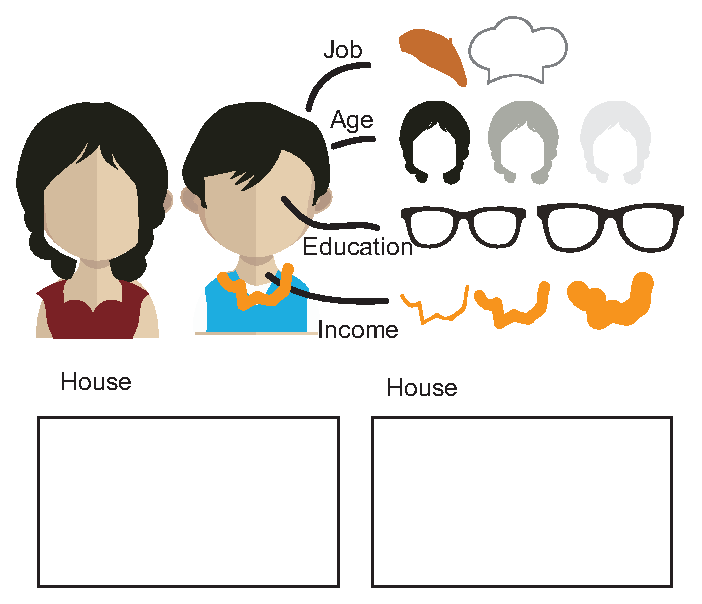
\includegraphics[width=\columnwidth]{pictures/design_profile}
 \caption{Design Profile}
 \label{fig:design_profile}
\end{figure}

With the visual mapping, the profiles varies from individual to individual. Figure~\ref{fig:div_profile} shows some examples. By concretizing the attributes which otherwise is too abstract to percept, users can scan and search for interesting target organically in figures.

\begin{figure}[htb!]
 \centering % avoid the use of \begin{center}...\end{center} and use \centering instead (more compact)
 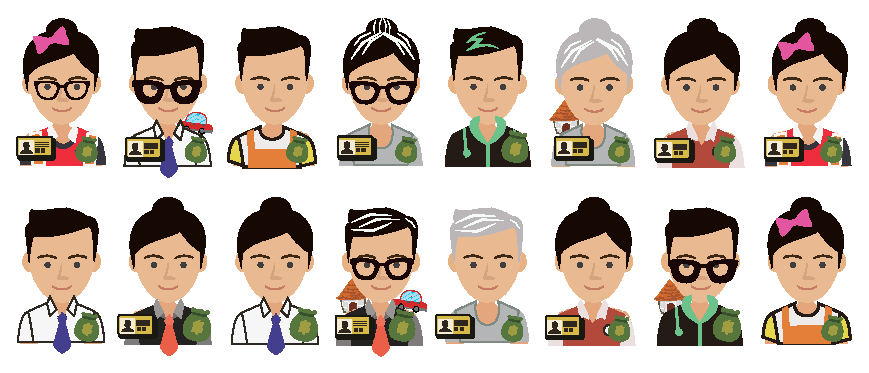
\includegraphics[width=\columnwidth]{pictures/design_div}
 \caption{Diverse Profile}
 \label{fig:div_profile}
\end{figure}

\subsection{t-SNE Projection}

Each individual is denoted as a vector with eight factors and projected as a dot into the 2D view via t-SNE project~\cite{maaten2008visualizing}, which well suits high-dimensional data for visualization in a low-dimensional space of two dimensions. As Figure~\ref{fig:tsne}(a)shows, all volunteers are embedded evenly in the 2D view, indicating the uniformly sampling over demographical space. 

Multiple views of abstract view, t-SNE proection and semantic data driven profile visualization are coordinated in a Cross-filter machinesm~\cite{Weaver2010}. It allows end-users to interactive drill-dowm into individuals with interested characteristics from multiple perspectives. Starting from the abstract criterion constraints, the scope of interest is narrowed down to individuals with(out) certian properties. And then further cross-filtering with semantically visual profiles, to check the combination of 8 characteristical variables. Figure~\ref{fig:tsne}(b) examplifies four groups of interest. 

\begin{figure}[htb!]
 \centering % avoid the use of \begin{center}...\end{center} and use \centering instead (more compact)
 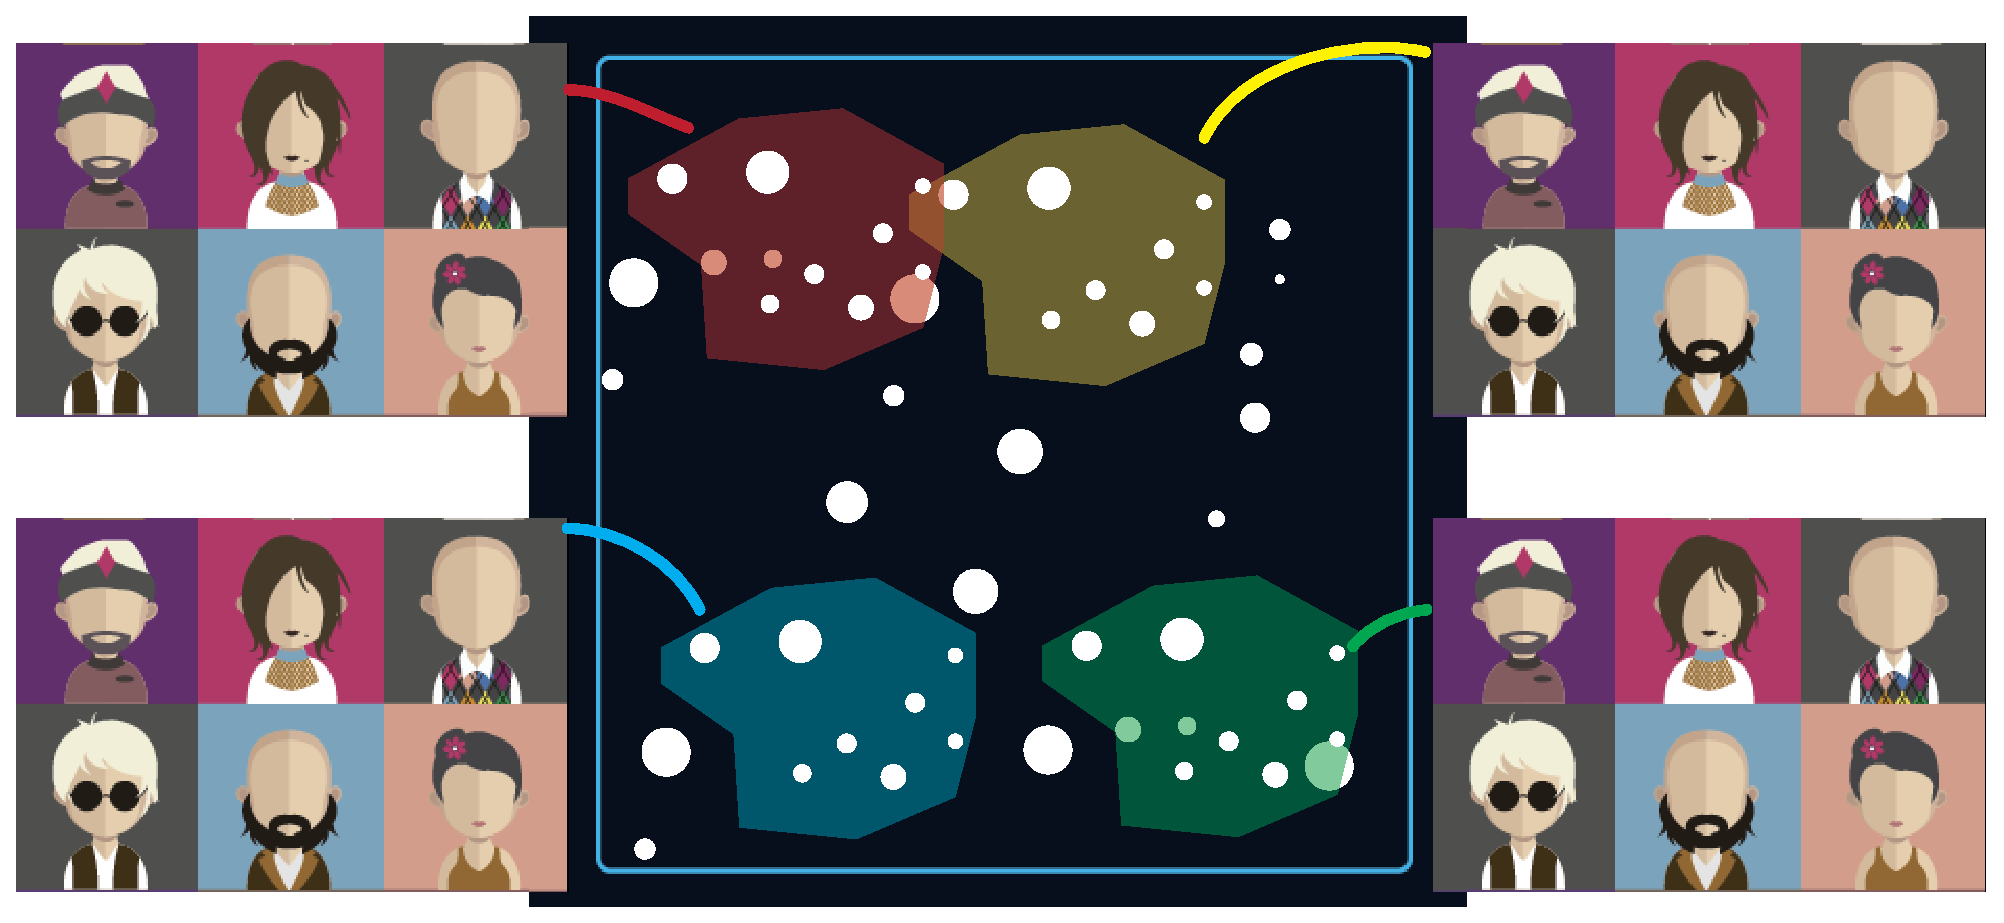
\includegraphics[width=\columnwidth]{pictures/mds}
 \caption{t-SNE project with four groups of the interest}
 \label{fig:tsne}
\end{figure}

\subsection{2.5D Spatial Visualization}

Embedding multiple variables in the spatial map is a challenging problem. Distortion technique 2D spatial, such as the partial route embedding~\cite{sun2016embedding}. However, when it comes to the global visualization, the trade-off between occlusion-free and the spatial perception. Follow the idea of 2.5D space design~\cite{Tominski2012_stacking}, the space visualization is embedded in 2.5D space, which also can smoothly transited back to the conventional 2D view.  

 Each TAZ is grown as a prism whose height encodes the occurrence of visiting. Brunch of TAZ with similar visiting pattern and purpose are grouped by an heuristic DB-Scan Algorithm in the context of TAZ. From a center TAZ, walk to neighbour TAZ to check whether aggregation or not. The aggregated TAZ brunch indicates the region visiting by the group of people in same purpose, which is often the popular traveling places. The TAZ brunch is visualized...

 To compare the mobility patterns across different groups of people, a Small Multiple dock is used to reserve the ever explored interesting result. To simply the comparion over spatial distribution, the snapshot is rendered in the 2D space, which can be magnified to check for the details in the 2.5D space.

 In this view, it supports end-users to direct manipulate the space, e.g., zooming, panning, etc. Also, detail information about the visiting can be checked by direct clicking on the TAZ. 
% \section{Experts Feedback}

\lmc{Add a section to introduce the domain experts' feedback}


\lm{We interview XX domain experts from the GIS field. XX of them are with ... The procedure went as following. We first introduce them the system an...}

\section{Case Study}

Applied the system to Shenzhen's dataset. We demonstrate the efficiency. 

\subsection{OVERVIEW Case 1: City Folding}

compare the distorted maps from various groups

Different different groups of people and see their patterns across the city.

Group 1 is defined as xxxxx. The popular visiting places

Wealthier people with better access to ... than poor people. 

\subsection{DETAIL Case 2: Look into Detail}

check the detail information of a group

To compare the Group 1 and Group 2, the similar places and different places...



% An example of a floating figure using the graphicx package.
% Note that \label must occur AFTER (or within) \caption.
% For figures, \caption should occur after the \includegraphics.
% Note that IEEEtran v1.7 and later has special internal code that
% is designed to preserve the operation of \label within \caption
% even when the captionsoff option is in effect. However, because
% of issues like this, it may be the safest practice to put all your
% \label just after \caption rather than within \caption{}.
%
% Reminder: the "draftcls" or "draftclsnofoot", not "draft", class
% option should be used if it is desired that the figures are to be
% displayed while in draft mode.
%
%\begin{figure}[!t]
%\centering
%\includegraphics[width=2.5in]{myfigure}
% where an .eps filename suffix will be assumed under latex, 
% and a .pdf suffix will be assumed for pdflatex; or what has been declared
% via \DeclareGraphicsExtensions.
%\caption{Simulation results for the network.}
%\label{fig_sim}
%\end{figure}

% Note that the IEEE typically puts floats only at the top, even when this
% results in a large percentage of a column being occupied by floats.
% However, the Computer Society has been known to put floats at the bottom.


% An example of a double column floating figure using two subfigures.
% (The subfig.sty package must be loaded for this to work.)
% The subfigure \label commands are set within each subfloat command,
% and the \label for the overall figure must come after \caption.
% \hfil is used as a separator to get equal spacing.
% Watch out that the combined width of all the subfigures on a 
% line do not exceed the text width or a line break will occur.
%
%\begin{figure*}[!t]
%\centering
%\subfloat[Case I]{\includegraphics[width=2.5in]{box}%
%\label{fig_first_case}}
%\hfil
%\subfloat[Case II]{\includegraphics[width=2.5in]{box}%
%\label{fig_second_case}}
%\caption{Simulation results for the network.}
%\label{fig_sim}
%\end{figure*}
%
% Note that often IEEE papers with subfigures do not employ subfigure
% captions (using the optional argument to \subfloat[]), but instead will
% reference/describe all of them (a), (b), etc., within the main caption.
% Be aware that for subfig.sty to generate the (a), (b), etc., subfigure
% labels, the optional argument to \subfloat must be present. If a
% subcaption is not desired, just leave its contents blank,
% e.g., \subfloat[].


% An example of a floating table. Note that, for IEEE style tables, the
% \caption command should come BEFORE the table and, given that table
% captions serve much like titles, are usually capitalized except for words
% such as a, an, and, as, at, but, by, for, in, nor, of, on, or, the, to
% and up, which are usually not capitalized unless they are the first or
% last word of the caption. Table text will default to \footnotesize as
% the IEEE normally uses this smaller font for tables.
% The \label must come after \caption as always.
%
%\begin{table}[!t]
%% increase table row spacing, adjust to taste
%\renewcommand{\arraystretch}{1.3}
% if using array.sty, it might be a good idea to tweak the value of
% \extrarowheight as needed to properly center the text within the cells
%\caption{An Example of a Table}
%\label{table_example}
%\centering
%% Some packages, such as MDW tools, offer better commands for making tables
%% than the plain LaTeX2e tabular which is used here.
%\begin{tabular}{|c||c|}
%\hline
%One & Two\\
%\hline
%Three & Four\\
%\hline
%\end{tabular}
%\end{table}


% Note that the IEEE does not put floats in the very first column
% - or typically anywhere on the first page for that matter. Also,
% in-text middle ("here") positioning is typically not used, but it
% is allowed and encouraged for Computer Society conferences (but
% not Computer Society journals). Most IEEE journals/conferences use
% top floats exclusively. 
% Note that, LaTeX2e, unlike IEEE journals/conferences, places
% footnotes above bottom floats. This can be corrected via the
% \fnbelowfloat command of the stfloats package.




\section{Conclusion}
\label{sec:conclusion}

Our analysis demonstrates how demographics survey collectd via social media have the potential to indiate the movement patterns of groups that have different social charactersitics and the difference in using urban facilities. Better understand of the interactions between population characteristics and their urban activity. The data we used represent a small propotion of the population of which we do not have the clear definition of its demographics. We consider this work as one of the first steps of research contextualize the analysis of urban dynamcis with social science, to understand the  interactions between population characteristics and their urban activity. 




% if have a single appendix:
%\appendix[Proof of the Zonklar Equations]
% or
%\appendix  % for no appendix heading
% do not use \section anymore after \appendix, only \section*
% is possibly needed

% use appendices with more than one appendix
% then use \section to start each appendix
% you must declare a \section before using any
% \subsection or using \label (\appendices by itself
% starts a section numbered zero.)
%


% \appendices
% \section{Proof of the First Zonklar Equation}
% Appendix one text goes here.

% you can choose not to have a title for an appendix
% if you want by leaving the argument blank
% \section{}
% Appendix two text goes here.


% use section* for acknowledgment
\ifCLASSOPTIONcompsoc
  % The Computer Society usually uses the plural form
  \section*{Acknowledgments}
\else
  % regular IEEE prefers the singular form
  \section*{Acknowledgment}
\fi


....


% Can use something like this to put references on a page
% by themselves when using endfloat and the captionsoff option.
\ifCLASSOPTIONcaptionsoff
  \newpage
\fi



% trigger a \newpage just before the given reference
% number - used to balance the columns on the last page
% adjust value as needed - may need to be readjusted if
% the document is modified later
%\IEEEtriggeratref{8}
% The "triggered" command can be changed if desired:
%\IEEEtriggercmd{\enlargethispage{-5in}}

% references section

% can use a bibliography generated by BibTeX as a .bbl file
% BibTeX documentation can be easily obtained at:
% http://mirror.ctan.org/biblio/bibtex/contrib/doc/
% The IEEEtran BibTeX style support page is at:
% http://www.michaelshell.org/tex/ieeetran/bibtex/
\bibliographystyle{IEEEtran}
% argument is your BibTeX string definitions and bibliography database(s)
\bibliography{main}
%
% <OR> manually copy in the resultant .bbl file
% set second argument of \begin to the number of references
% (used to reserve space for the reference number labels box)
%\begin{thebibliography}{1}

%\bibitem{IEEEhowto:kopka}
%H.~Kopka and P.~W. Daly, \emph{A Guide to \LaTeX}, 3rd~ed.\hskip 1em plus
%  0.5em minus 0.4em\relax Harlow, England: Addison-Wesley, 1999.

%\end{thebibliography}

% biography section
% 
% If you have an EPS/PDF photo (graphicx package needed) extra braces are
% needed around the contents of the optional argument to biography to prevent
% the LaTeX parser from getting confused when it sees the complicated
% \includegraphics command within an optional argument. (You could create
% your own custom macro containing the \includegraphics command to make things
% simpler here.)
%\begin{IEEEbiography}[{\includegraphics[width=1in,height=1.25in,clip,keepaspectratio]{mshell}}]{Michael Shell}
% or if you just want to reserve a space for a photo:


% You can push biographies down or up by placing
% a \vfill before or after them. The appropriate
% use of \vfill depends on what kind of text is
% on the last page and whether or not the columns
% are being equalized.

%\vfill

% Can be used to pull up biographies so that the bottom of the last one
% is flush with the other column.
%\enlargethispage{-5in}



% that's all folks
\end{document}


